\documentclass{article}\usepackage[]{graphicx}\usepackage[]{xcolor}
% maxwidth is the original width if it is less than linewidth
% otherwise use linewidth (to make sure the graphics do not exceed the margin)
\makeatletter
\def\maxwidth{ %
  \ifdim\Gin@nat@width>\linewidth
    \linewidth
  \else
    \Gin@nat@width
  \fi
}
\makeatother

\definecolor{fgcolor}{rgb}{0.345, 0.345, 0.345}
\newcommand{\hlnum}[1]{\textcolor[rgb]{0.686,0.059,0.569}{#1}}%
\newcommand{\hlsng}[1]{\textcolor[rgb]{0.192,0.494,0.8}{#1}}%
\newcommand{\hlcom}[1]{\textcolor[rgb]{0.678,0.584,0.686}{\textit{#1}}}%
\newcommand{\hlopt}[1]{\textcolor[rgb]{0,0,0}{#1}}%
\newcommand{\hldef}[1]{\textcolor[rgb]{0.345,0.345,0.345}{#1}}%
\newcommand{\hlkwa}[1]{\textcolor[rgb]{0.161,0.373,0.58}{\textbf{#1}}}%
\newcommand{\hlkwb}[1]{\textcolor[rgb]{0.69,0.353,0.396}{#1}}%
\newcommand{\hlkwc}[1]{\textcolor[rgb]{0.333,0.667,0.333}{#1}}%
\newcommand{\hlkwd}[1]{\textcolor[rgb]{0.737,0.353,0.396}{\textbf{#1}}}%
\let\hlipl\hlkwb

\usepackage{framed}
\makeatletter
\newenvironment{kframe}{%
 \def\at@end@of@kframe{}%
 \ifinner\ifhmode%
  \def\at@end@of@kframe{\end{minipage}}%
  \begin{minipage}{\columnwidth}%
 \fi\fi%
 \def\FrameCommand##1{\hskip\@totalleftmargin \hskip-\fboxsep
 \colorbox{shadecolor}{##1}\hskip-\fboxsep
     % There is no \\@totalrightmargin, so:
     \hskip-\linewidth \hskip-\@totalleftmargin \hskip\columnwidth}%
 \MakeFramed {\advance\hsize-\width
   \@totalleftmargin\z@ \linewidth\hsize
   \@setminipage}}%
 {\par\unskip\endMakeFramed%
 \at@end@of@kframe}
\makeatother

\definecolor{shadecolor}{rgb}{.97, .97, .97}
\definecolor{messagecolor}{rgb}{0, 0, 0}
\definecolor{warningcolor}{rgb}{1, 0, 1}
\definecolor{errorcolor}{rgb}{1, 0, 0}
\newenvironment{knitrout}{}{} % an empty environment to be redefined in TeX

\usepackage{alltt}
\usepackage{hyperref}
\usepackage{booktabs}
\usepackage[top=1.5cm, bottom=1.5cm, left=2cm, right=2cm]{geometry}
\IfFileExists{upquote.sty}{\usepackage{upquote}}{}
\begin{document}
% \SweaveOpts{concordance=TRUE}

\title{Results outline corintreespotters}
\author{Christophe Rouleau-Desrochers}
\date{\today}
\maketitle

% Set CoringTreespotters species shortcut
\newcommand{\Arub}{\textit{A. rubrum}}
\newcommand{\Asac}{\textit{A. saccharum}}
\newcommand{\Afla}{\textit{A. flava}}
\newcommand{\Ball}{\textit{B. alleghaniensis}}
\newcommand{\Bnig}{\textit{B. nigra}}
\newcommand{\Cgla}{\textit{C. glabra}}
\newcommand{\Cova}{\textit{C. ovata}}
\newcommand{\Pdel}{\textit{P. deltoides}}
\newcommand{\Qalb}{\textit{Q. alba}}
\newcommand{\Qrub}{\textit{Q. rubra}}
\newcommand{\Tame}{\textit{T. americana}}   


\begin{knitrout}
\definecolor{shadecolor}{rgb}{0.969, 0.969, 0.969}\color{fgcolor}

\includegraphics[width=\maxwidth]{figure/setup-1} 
\begin{kframe}

{\ttfamily\noindent\bfseries\color{errorcolor}{\#\# Error in `h()`:\\\#\# ! error in evaluating the argument 'y' in selecting a method for function 'plot': object 'y\_pos' not found}}\end{kframe}
\end{knitrout}

% <><><><><><><><><><><><><><><><><><><><><><><><><><><><><><><><><><><><><><><>
\section*{Research questions}
% <><><><><><><><><><><><><><><><><><><><><><><><><><><><><><><><><><><><><><><>
\begin{enumerate}
\item Does tree growth increase with longer growing seasons?
\item Did an earlier start and later end of season increase growth? 
\item Does tree growth increase with longer growing seasons and is it consistent across species?
\item How did growth change across years, and how did it relate to climate?
\end{enumerate}

% <><><><><><><><><><><><><><><><><><><><><><><><><><><><><><><><><><><><><><><>
\section*{Results}
% <><><><><><><><><><><><><><><><><><><><><><><><><><><><><><><><><><><><><><><>

\begin{enumerate}
\item CoringTreespotters includes eleven deciduous tree species with phenological observations from 2016 to 2024. In total, our final dataset has 329 leafout observations and 
310 leaf coloring observations. We used these phenophases to set the boundaries of individual-level growing seasons, which together yield 
280 complete growing seasons.
\end{enumerate}

\begin{enumerate}
\item Summary basic information
  \begin{enumerate}
  \item Coringtreespotters includes eleven with leaf phenology data spaning nine years (2016 to 2024) for a total of 329 leafout and 310 colored leaves observations, yielding 280 complete growing seasons (GS) for 49 individuals. 
    \item GSL ranged from 
  77 days ({\Afla} in 2018) to 
  194 days ({\Asac} in 2021)

  \item GS thermal sum ranged from 
  1048.8 GDD ({\Afla} in 2020) to 
  2634.7 GDD, ({\Tame} in 2016)
  
  \item The earliest leafout day of year was 08-Apr (2021) and the latest, 14-Jun (2021). The earliest coloredLeaves day of year was 15-Jul (2021) and the latest, 06-Nov (2021) 
  
  \item 2018 had a mean summer temperature of 22.85$^\circ$C and had a mean summer PDSI value of
  1.92. 2019 was cooler
  (22.38$^\circ$C) and wetter
  (PDSI $=$ 4.02), whereas 2020 was warmer
  (23.07$^\circ$C) and drier
  (PDSI $=$ -2.35) than 2018.

\end{enumerate}

% Question 1 --- --- --- --- --- --- --- --- --- --- --- --- --- --- --- --- ---
\item Does tree growth increase with longer growing seasons?
  \begin{enumerate}

  \item No clear trend of growing season length effect across our eleven species and season predictors.

  \item Longer thermal season increased growth *weakly for \Asac ($\beta = $
  0.09, $UI_{90}$
  [-0.02,
  0.2]), \Bnig  ($\beta = $
  0.08, $UI_{90}$
  [-0.01,
  0.16]), \Cgla ($\beta = $
  0.05, $UI_{90}$
  [-0.06,
  0.17]), \Qrub ($\beta = $
  0.08, $UI_{90}$
  [-0.09,
  0.26]), and decreased for {\Ball} ($\beta = $
  -0.22, $UI_{90}$
  [-0.36,
  -0.09])
  ) (Figure \ref{fig:tsmuplotbsppTS}a and e) (Table \ref{tab:ts_slope_table}). 
 
  \item Of the four species that grew more with longer thermal season all, only two also grew more with longer   calendar season (\Bnig: $\beta = $
  0.03, $UI_{90}$
  [-0.02,
  0.07], \Cgla: $\beta = $
  0.03, $UI_{90}$
  [-0.03,
  0.08]), and {\Tame} growth decreased   ($\beta = $
  -0.02, $UI_{90}$
  [-0.05,
  0.01]), unlike its response to
  the thermal season. 

  \item \Ball trended in the same direction, but showed a weaker reponse than the thermal season ($\beta = $
  -0.05, $UI_{90}$
  [-0.11,
  0.02]) 
   (Figure \ref{fig:tsmuplotbsppTS}b and f) (Table \ref{tab:ts_slope_table}). 
   (Figure \ref{fig:buburstVSleafoutTS}b).
  
  \item Results with basal area increment (BAI) for the GDD model were broadly similar to ring width (see Figure \ref{fig:RWvsBAI} and Table \ref{tab:BAItab})
  \end{enumerate}
  
% Question 2 --- --- --- --- --- --- --- --- --- --- --- --- --- --- --- --- ---
\item Did a later start and end of season increase growth?
  \begin{enumerate}
  \item A later start of season increased growth for {\Tame} ($\beta = $
  0.14, $UI_{90}$
  [0.01,
  0.26]), but \Asac: $\beta = $
  0.07, $UI_{90}$
  [-0.02,
  0.16], \Bnig: $\beta = $
  0.03,   $UI_{90}$
  [-0.1,
  0.16], \Cgla: $\beta = $
  0.07, $UI_{90}$
  [-0.09,
  0.22], \Cova: $\beta = $
  0.09, $UI_{90}$
  [-0.04,
  0.22], \Pdel: $\beta = $
  0.06, $UI_{90}$
  [-0.08,
  0.2], \Qrub: $\beta = $
  0.08, $UI_{90}$
  [-0.09,
  0.26] trended in the same direction, and \Ball ($\beta = $
  -0.07,   $UI_{90}$
  [-0.22,
  0.07]) trended in the opposite direction
  (Figure \ref{fig:tsmuplotbsppTS}c and g) (Table \ref{tab:ts_slope_table}). 

\item A later end of season decreased growth for {\Ball} ($\beta = $
-0.08, $UI_{90}$[-0.15,
-0.01]), but \Tame ($\beta = $
-0.01, $UI_{90}$[-0.04,
0.02]) trended towards the same direction and {\Asac} ($\beta = $
0.03, $UI_{90}$
[-0.03,
0.08], {\Bnig} ($\beta = $
0.03, $UI_{90}$[-0.02,
0.08]), and \Cgla: $\beta = $
0.03, $UI_{90}$
[-0.02,
0.09] trended towards an increase in growth.
(Figure \ref{fig:tsmuplotbsppTS}d and h) (Table \ref{tab:ts_slope_table}). 

% The estimates were unchanged when using the full ($n =$nrow(empfulleosts)) or restricted datasets ($n=$nrow(empts)) (Figure \ref{fig:tsSOSEOScomparison}b).

% \item The estimates were unchanged when using the full or restricted datasets ($n =$
% nrow(empfullsosts) vs $n=$
% nrow(empts) Figure \ref{fig:tsSOSEOScomparison}b), or when using budburst instead of leafout as the start of the growing season (Figure \ref{fig:buburstVSleafoutTS}c).
  
  \end{enumerate}

% Question 3 --- --- --- --- --- --- --- --- --- --- --- --- --- --- --- --- ---
% \item Does tree growth increase with longer growing seasons and is it consistent across species and provenances?
%   \begin{enumerate}
%   
%   \item {\Ball} grew the most, and was the most responsive to longer growing seasons
%   
%   \item {\Bpap} grew the least ($\alpha = $ 
%   aspp_df2$mean[which(aspp_df2$spp_name %in% "B. papyrifera")], $UI_{90}$
%   [aspp_df2$p5[which(aspp_df2$spp_name %in% "B. papyrifera")], 
%   aspp_df2$p95[which(aspp_df2$spp_name %in% "B. papyrifera")]]) (Figure \ref{fig:tsmuplotatreeid}), but was the most responsive to longer growing seasons (Figure \ref{fig:tsmuplotbspp}a and b).
%   
%   \item {\Ainc} grew the most ($\alpha = $  
%   aspp_df2$mean[which(aspp_df2$spp_name %in% "A. incana")], $UI_{90}$
%   [aspp_df2$p5[which(aspp_df2$spp_name %in% "A. incana")], 
%   aspp_df2$p95[which(aspp_df2$spp_name %in% "A. incana")]]) (Figure \ref{fig:tsmuplotatreeid}), but had contrasting responses to longer growing seasons (Figure \ref{fig:tsmuplotbspp}a and b).
% 
%   \item Growth did not change across any provenances (Figure \ref{fig:tsmuplotasite}) (Table \ref{tab:ts_asite_table}), but there was slightly more variation across sites ($\sigma = $
%   sigma_df2$mean[which(sigma_df2$sigma %in% "sigma_asite")], $UI_{90}$
%   [sigma_df2$p5[which(sigma_df2$sigma %in% "sigma_asite")], 
%   sigma_df2$p95[which(sigma_df2$sigma %in% "sigma_asite")]) than across tree ids ($\sigma = $ 
%   sigma_df2$mean[which(sigma_df2$sigma %in% "sigma_atreeid")], $UI_{90}$
%   [sigma_df2$p5[which(sigma_df2$sigma %in% "sigma_atreeid")], 
%   sigma_df2$p95[which(sigma_df2$sigma %in% "sigma_atreeid")]]
% 
%   \end{enumerate}


% Question 4 --- --- --- --- --- --- --- --- --- --- --- --- --- --- --- --- ---
% \item How did growth change across years, and how did it relate to climate?
%   \begin{enumerate}
%   
%   \item Annual ring widths across years varied from 
%   min(empts$lengthMM) mm ({\Ball} in empts$year[which.min(empts$lengthMM)]) to 
%   max(empts$lengthMM) mm ({\Bpop} in empts$year[which.max(empts$lengthMM)]) (Figure \ref{fig:tsmuplotayear}). 
%  
%   \item Growth was highest in ayear_df2$year_name[which.max(ayear_df2$mean)] 
%   (ayear_df2$mean[which.max(ayear_df2$mean)], $UI_{90}$
%   [ayear_df2$p5[which.max(ayear_df2$mean)], 
% ayear_df2$p95[which.max(ayear_df2$mean)]]) (Figure \ref{fig:tsmuplotayear}), but that year was not the warmest nor the longest calendar season, unlike our finding that warmer and longer seasons increase growth for most of our species (Figure \ref{fig:tsxyGDD} and Figure \ref{fig:tsxyGSL}).
%   
%   \item Growth was lowest in ayear_df2$year_name[which.min(ayear_df2$mean)] 
%   (ayear_df2$mean[which.min(ayear_df2$mean)], $UI_{90}$
%   [ayear_df2$p5[which.min(ayear_df2$mean)], 
%   ayear_df2$p95[which.min(ayear_df2$mean)]]) (Figure \ref{fig:tsmuplotayear}) that year had the warmest thermal, but the shortest calendar season, also unlike our findings that growth increases with warmer seasons, and to a lesser extent, with longer calendar season (Figure \ref{fig:tsxyGDD} and Figure \ref{fig:tsxyGSL}).
%   \end{enumerate}
% 
% \end{enumerate}

% Figure mu across all species and climate predictors
\begin{figure}[!ht]
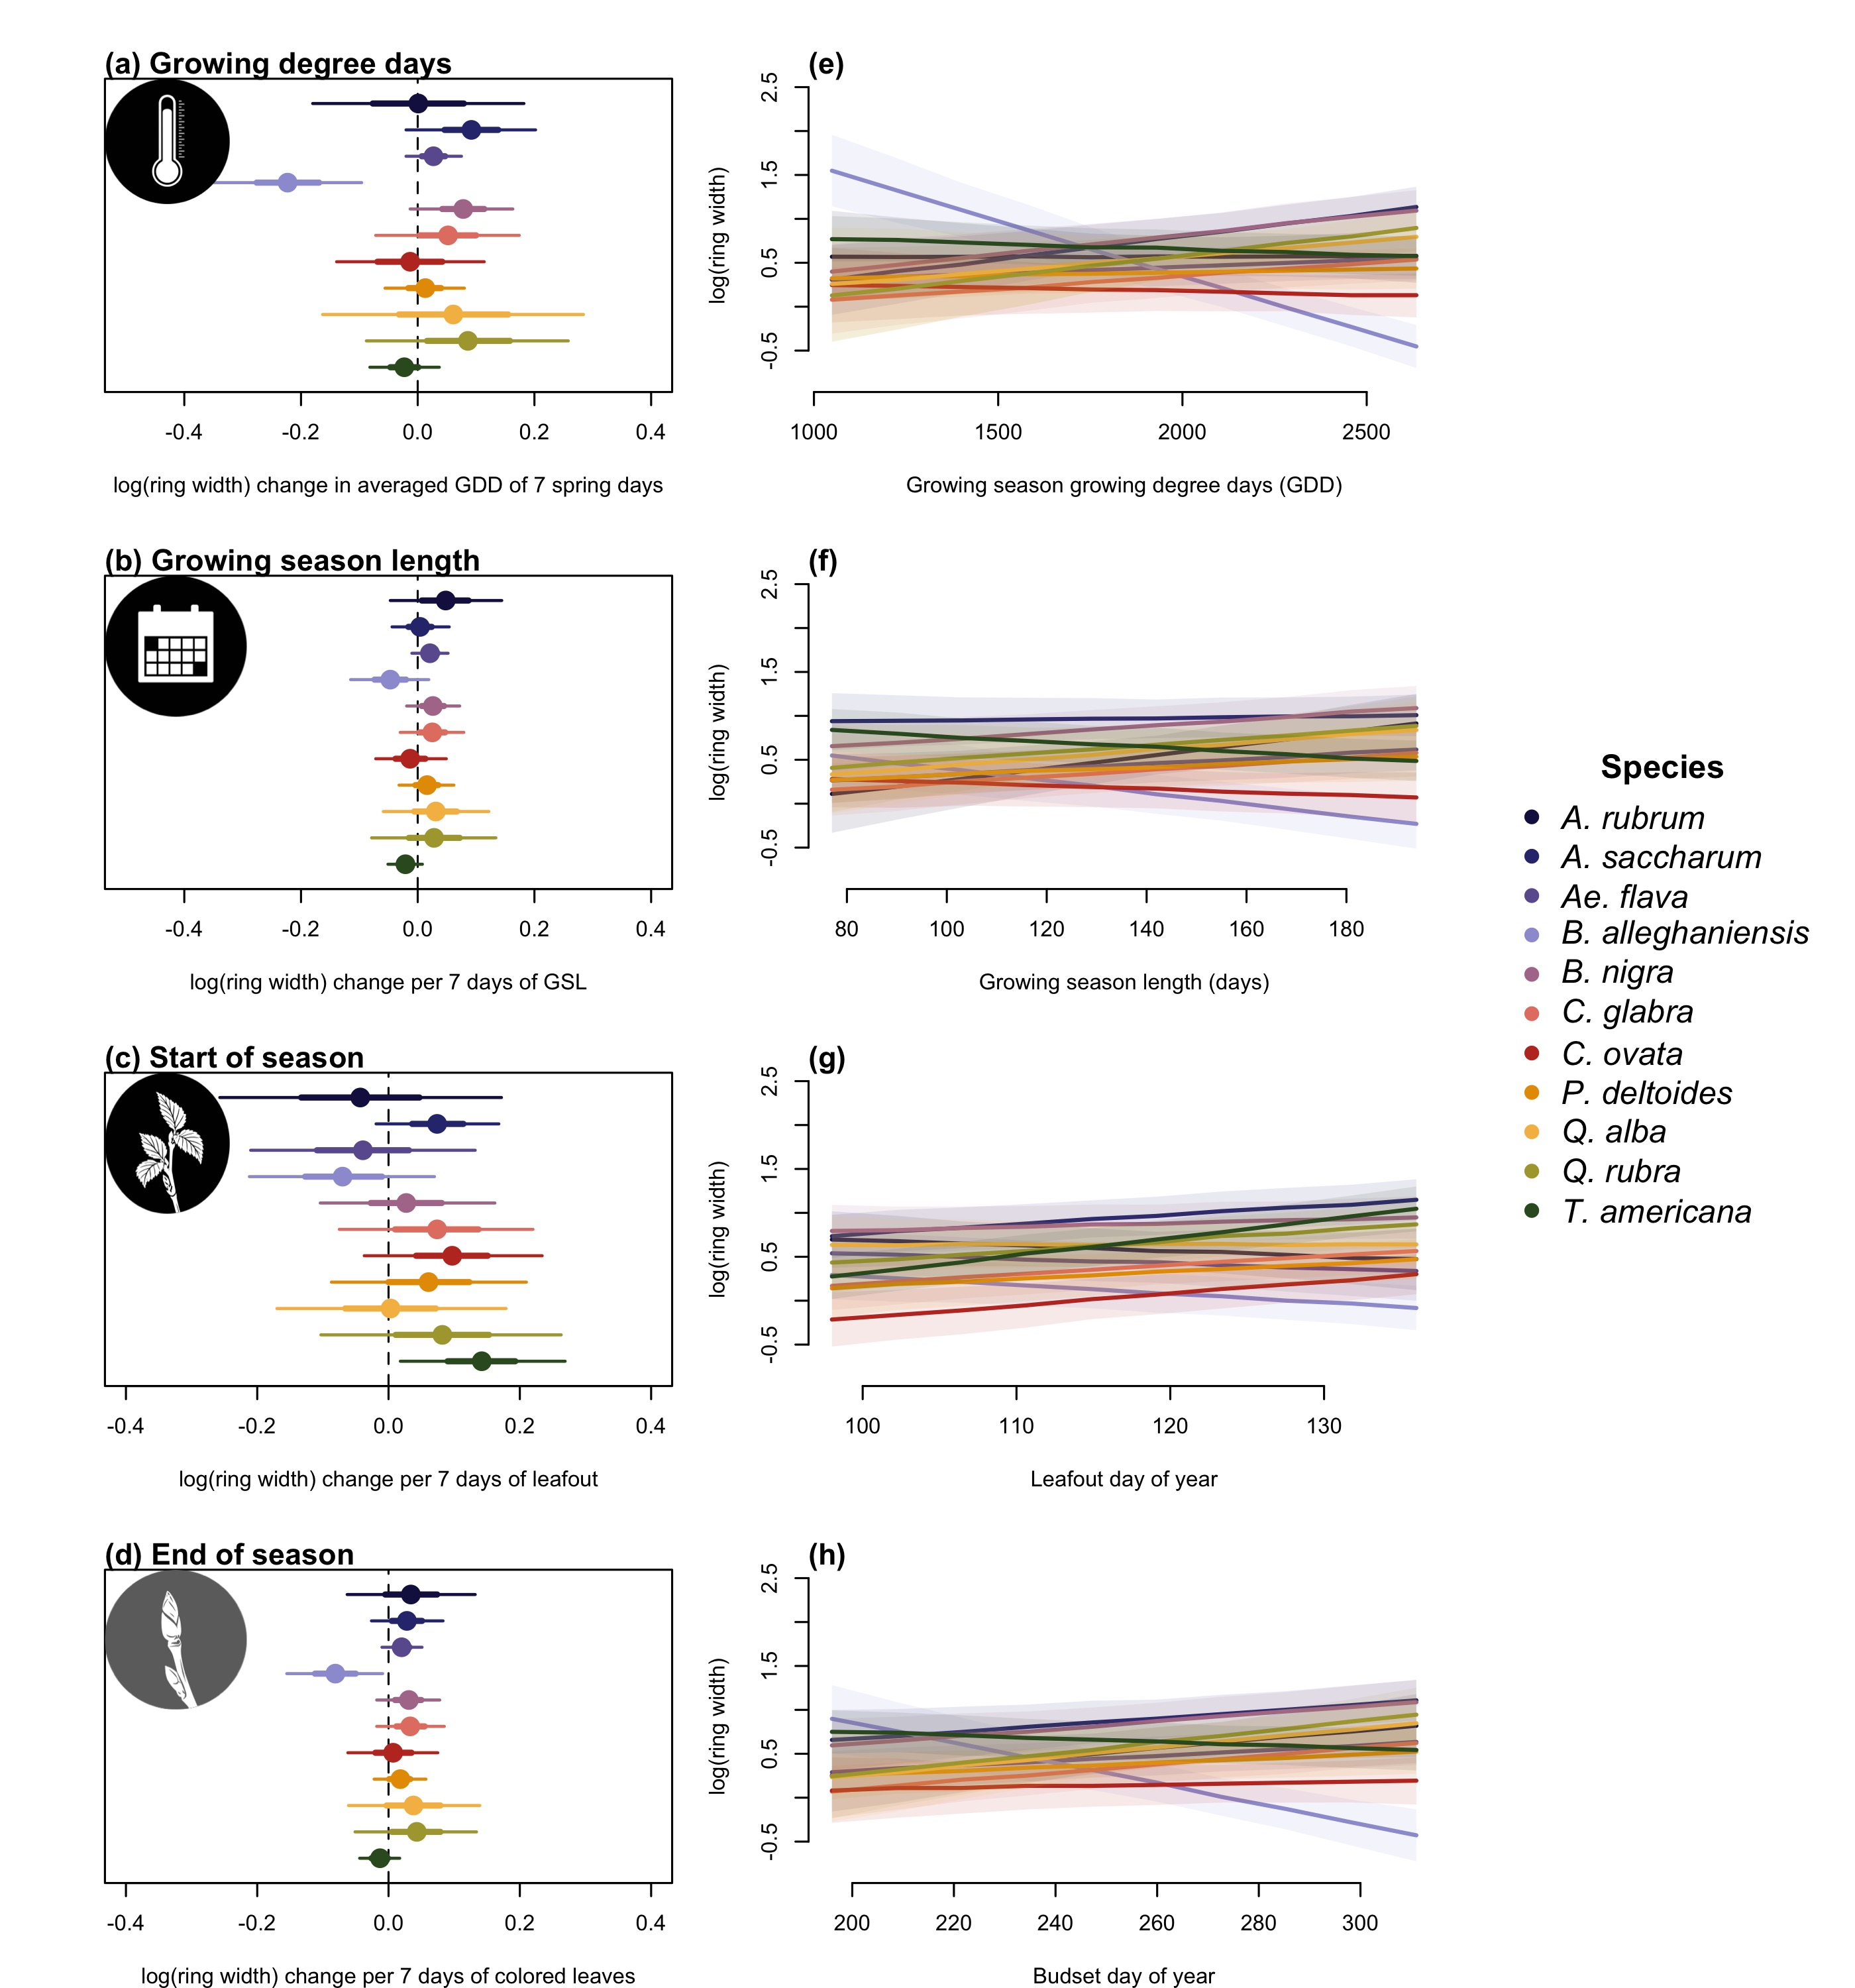
\includegraphics[width=0.8\textwidth]{../../analyses/figures/growthModelsMain/TSmuALLbsppWlines.jpeg}
\caption{Model slope estimates representing ring width change as a function of four different predictors across four species. GDD represent the accumulated growing degree days between leafout and coloredLeaves and the models estimates shows ring width change per 7 average spring days GDD (176.87) (a). GSL is the number of days between leafout and coloredLeaves (b). SOS represent the start of season, which is leafout (c) and EOS, the end of season through coloredLeaves (d). All predictors were fit using the same model and number of observations, with only the independent variable changing. The dots represent the mean of each species and the lines, the 50\% and 90\% uncertainty intervals (UI). 
% {\Ainc} and {\Bpap} grew more with longer calendar seasons, but only {\Ainc} grew less with later leafout and had no effect in response to coloredLeaves. Interestingly, {\Bpap} did not grow more with earlier leafout, but did with a later coloredLeaves and longer calendar season. {\Ball} and {\Bpop} did not grow more with longer calendar seasons, but {\Ball} grew more with a later leafout and coloredLeaves whereas {\Bpop} only grew more with a later coloredLeaves.
}
\label{fig:tsmuplotbspp}
\end{figure}

% Coringtreespotters year mu plot
\begin{figure}[!ht]
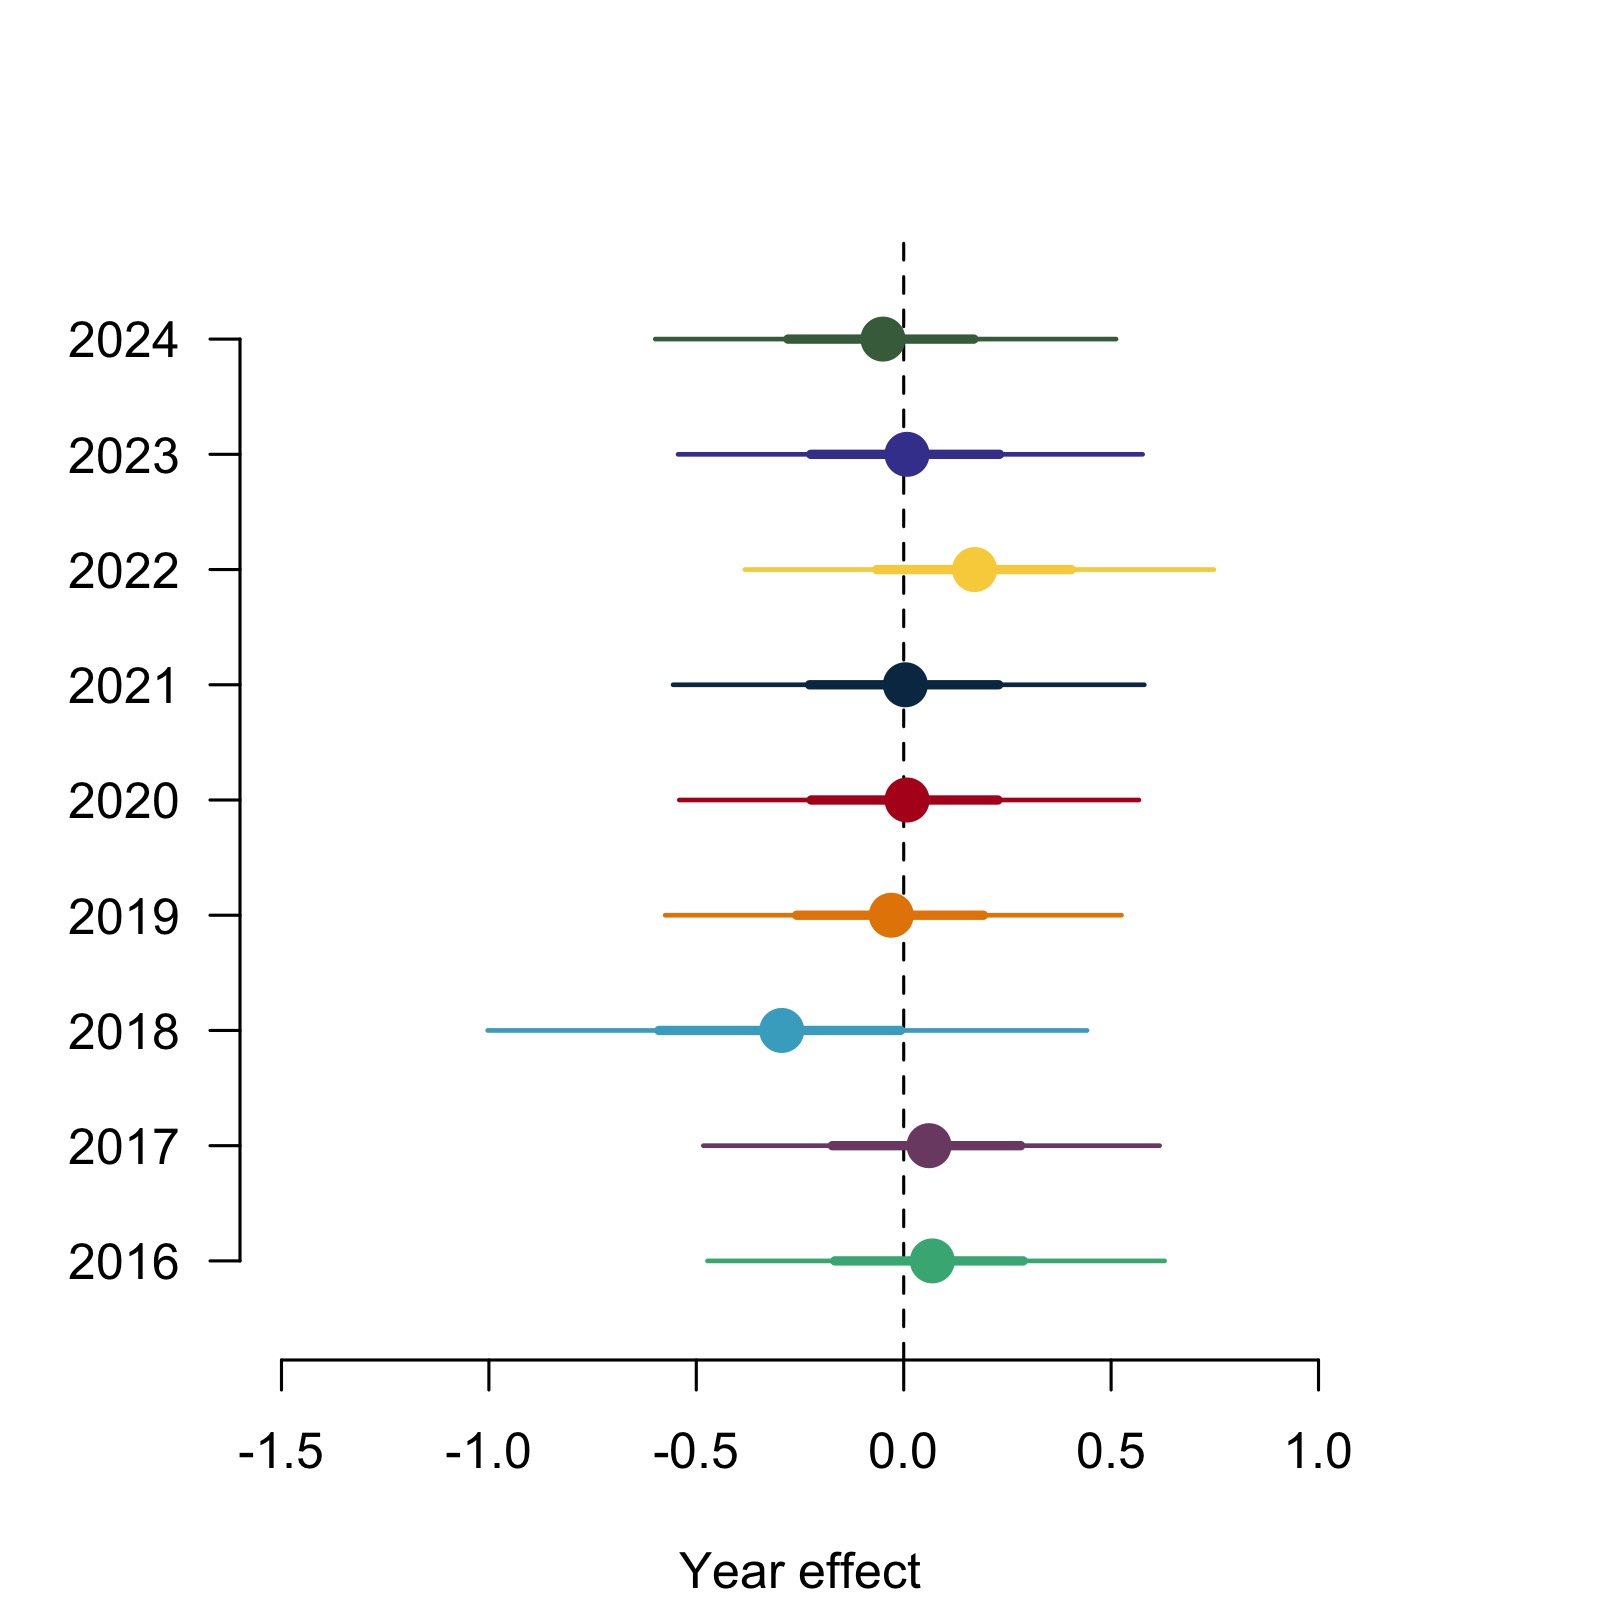
\includegraphics[width=1\textwidth]{../../analyses/figures/growthModelsMain/TSmuayear.jpeg}
\caption{We show tree ring widths (mm) across years as model estimates for the year intercepts with the dots depicting the mean and the lines, the 50\% and 90\% uncertainty intervals (UI).}
\label{fig:tsmuplotayear}
\end{figure}


% <><><><><><><><><><><><><><><><><><><><><><><><><><><><><><><><><><><><><><><>
% Supplemental results
% <><><><><><><><><><><><><><><><><><><><><><><><><><><><><><><><><><><><><><><>
\clearpage
\section*{Supplemental results}

\setcounter{table}{0}
\renetsommand{\thetable}{S\arabic{table}}
\setcounter{figure}{0}
\renetsommand{\thefigure}{S\arabic{figure}}

% Table slope for Coringtreespotters


% XY facetted by species GDD
\begin{figure}[!ht]
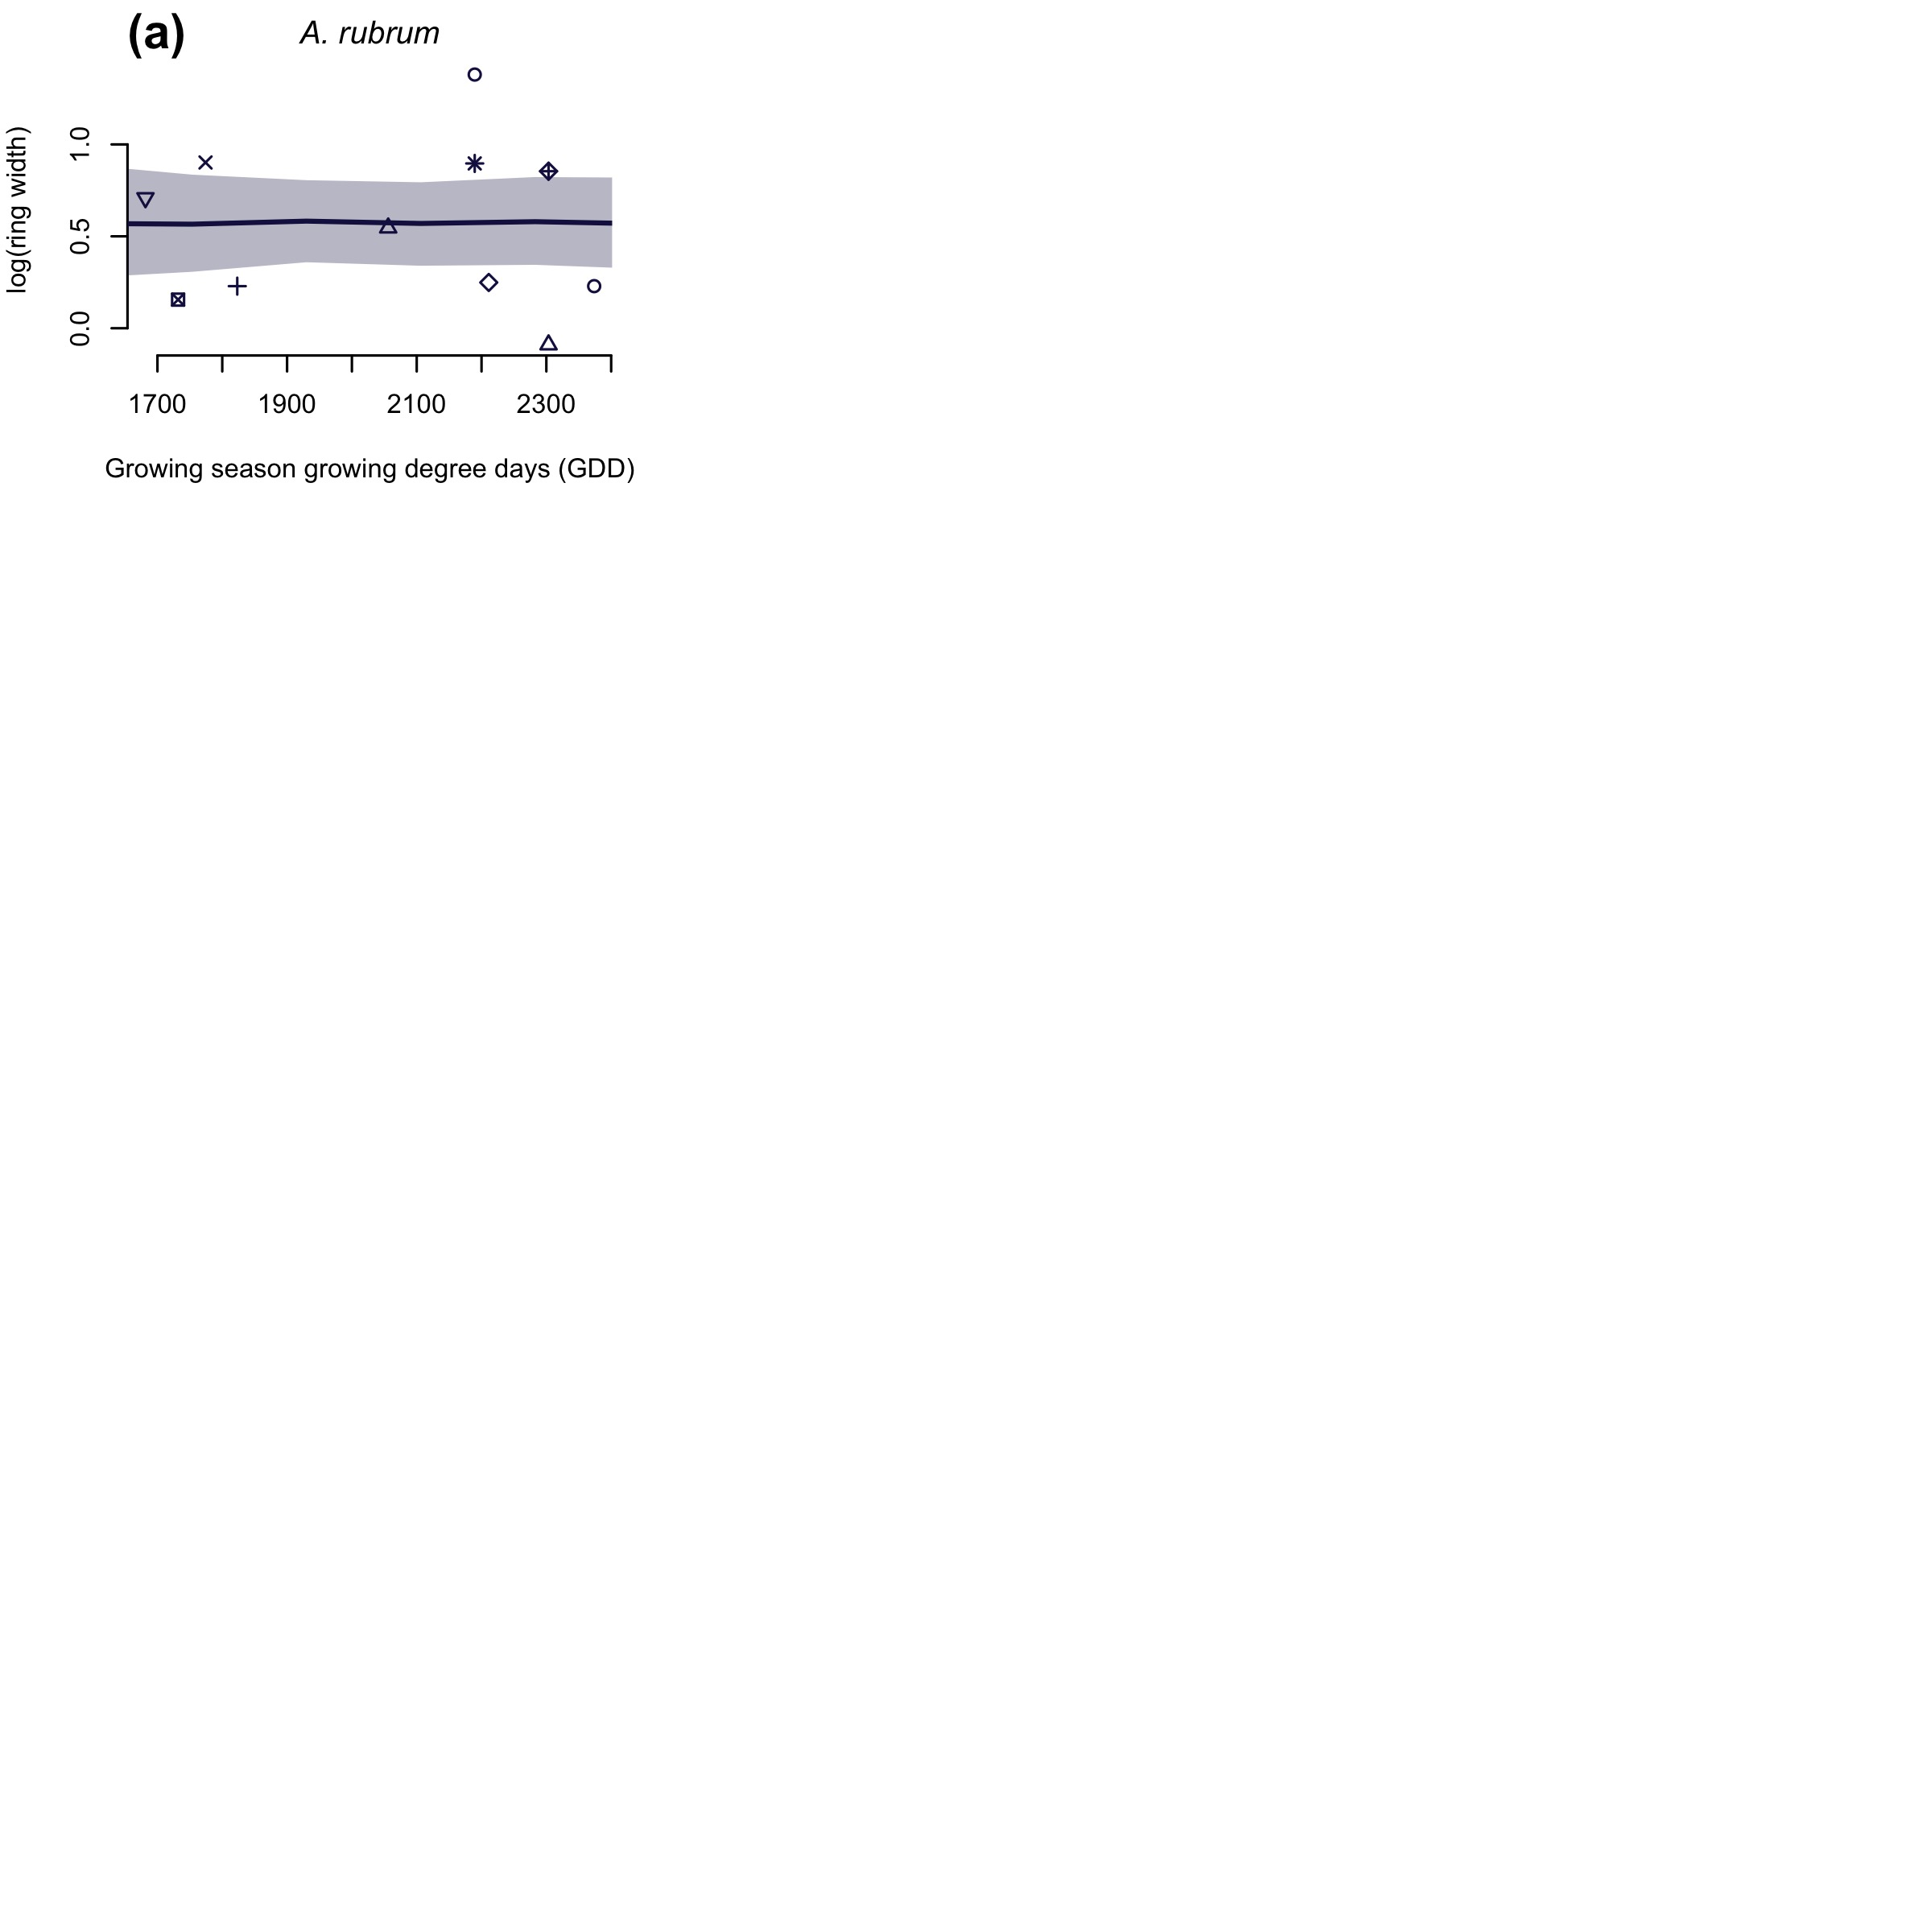
\includegraphics[width=0.8\textwidth]{../../analyses/figures/growthModelsMain/TSgrowthModelSlopesperSppFacetGDD.jpeg}
\caption{Ring width trends in response to thermal season (GDD). The plots are the reconstructed species estimates posterior distribution with error. The lines represent the mean of the posterior distribution and the shaded area, the 50\% UI. The dots are the empirical data shaped by year.}
\label{fig:tsxyGDD}
\end{figure}

% XY facetted by species GSL
\begin{figure}[!ht]
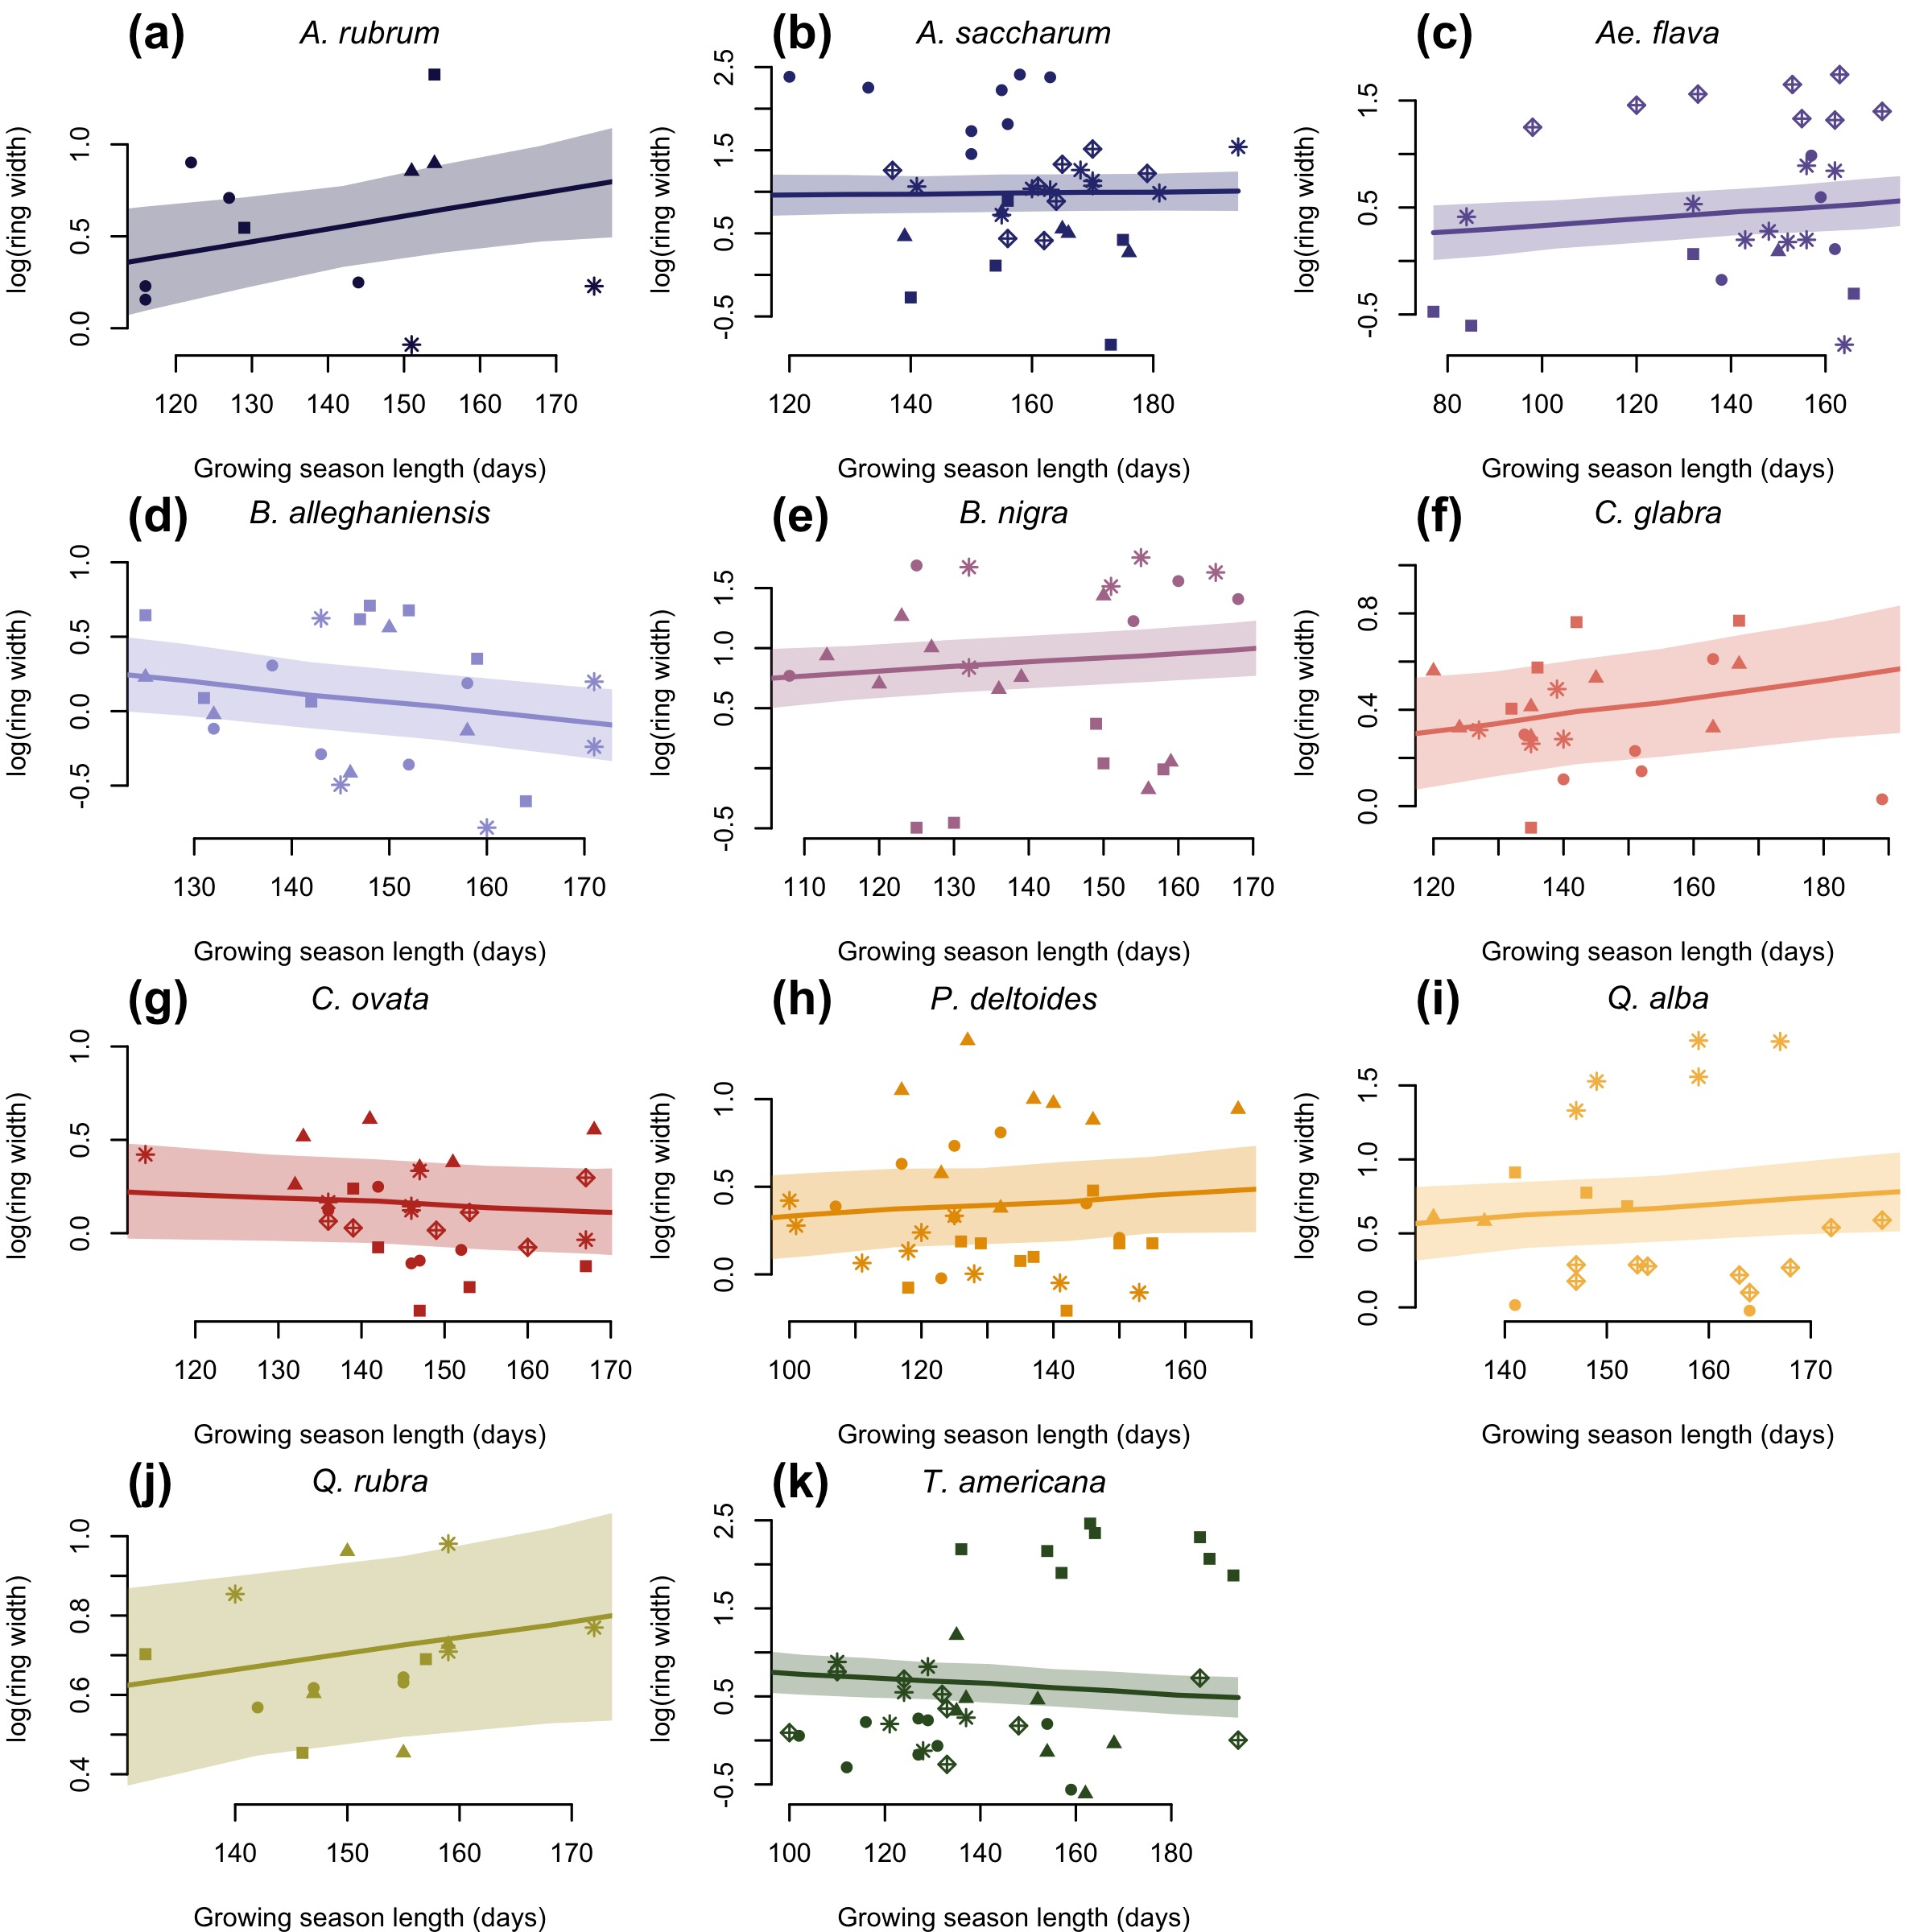
\includegraphics[width=0.8\textwidth]{../../analyses/figures/growthModelsMain/TSgrowthModelSlopesperSppFacetGSL.jpeg}
\caption{Ring width trends in response to calendar season (GSL). The plots are the reconstructed species estimates posterior distribution with error. The lines represent the mean of the posterior distribution and the shaded area, the 50\% UI. The dots are the empirical data shaped by year.}
\label{fig:tsxyGSL}
\end{figure}

% Figure mu atreeid full
\begin{figure}[!ht]
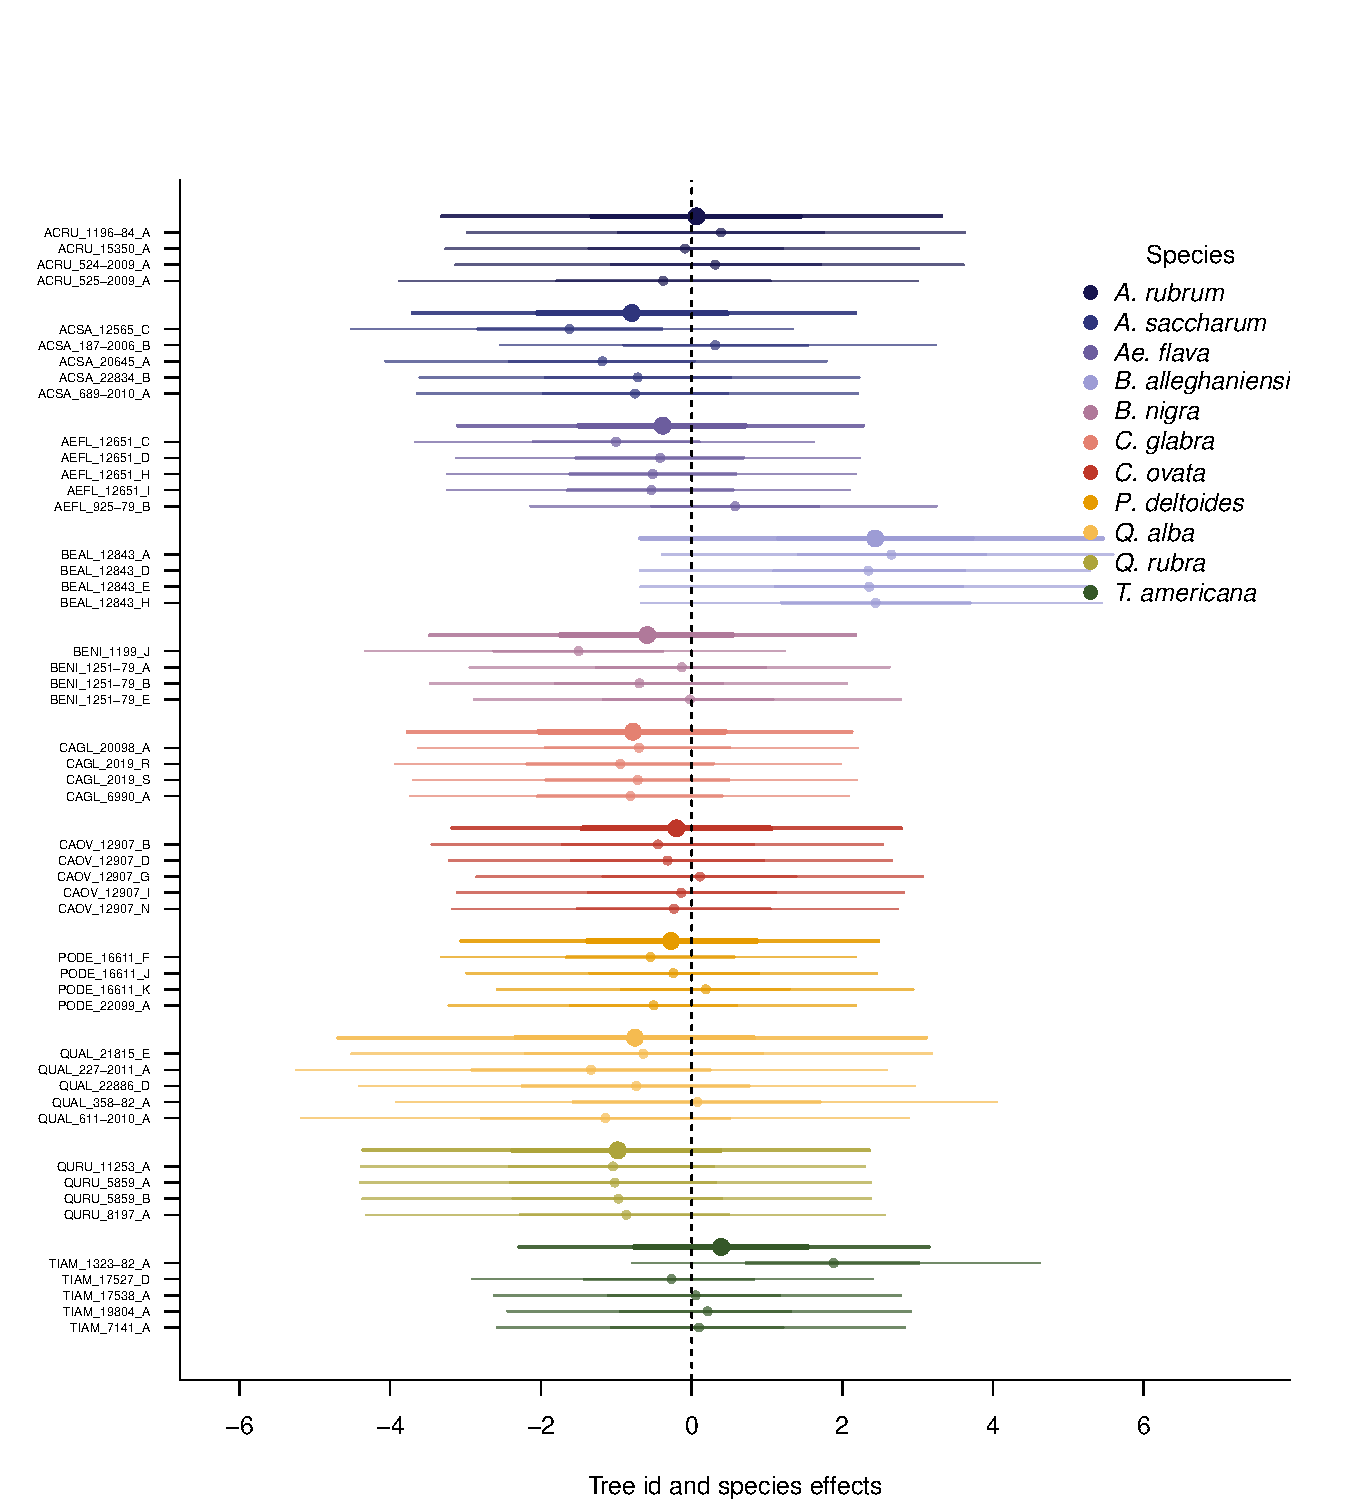
\includegraphics[width=0.8\textwidth]{../../analyses/figures/growthModelsMain/TSmeanPlotGrowthGDD_treeidBYspp.pdf}
\caption{Intercept estimates for each group of the GDD model. The different tree id values represent the sum of the tree id, provenance, species and averaged year intercepts. The larger dots and lines represent aggregated average across these values. The dots are the mean of the posterior distribution and the thick and thin lines, the 50 and 90\% UI.}
\label{fig:tsmuplotatreeid}
\end{figure}

% Z-scored slope results Coringtreespotters
% \begin{figure}[!ht]
% 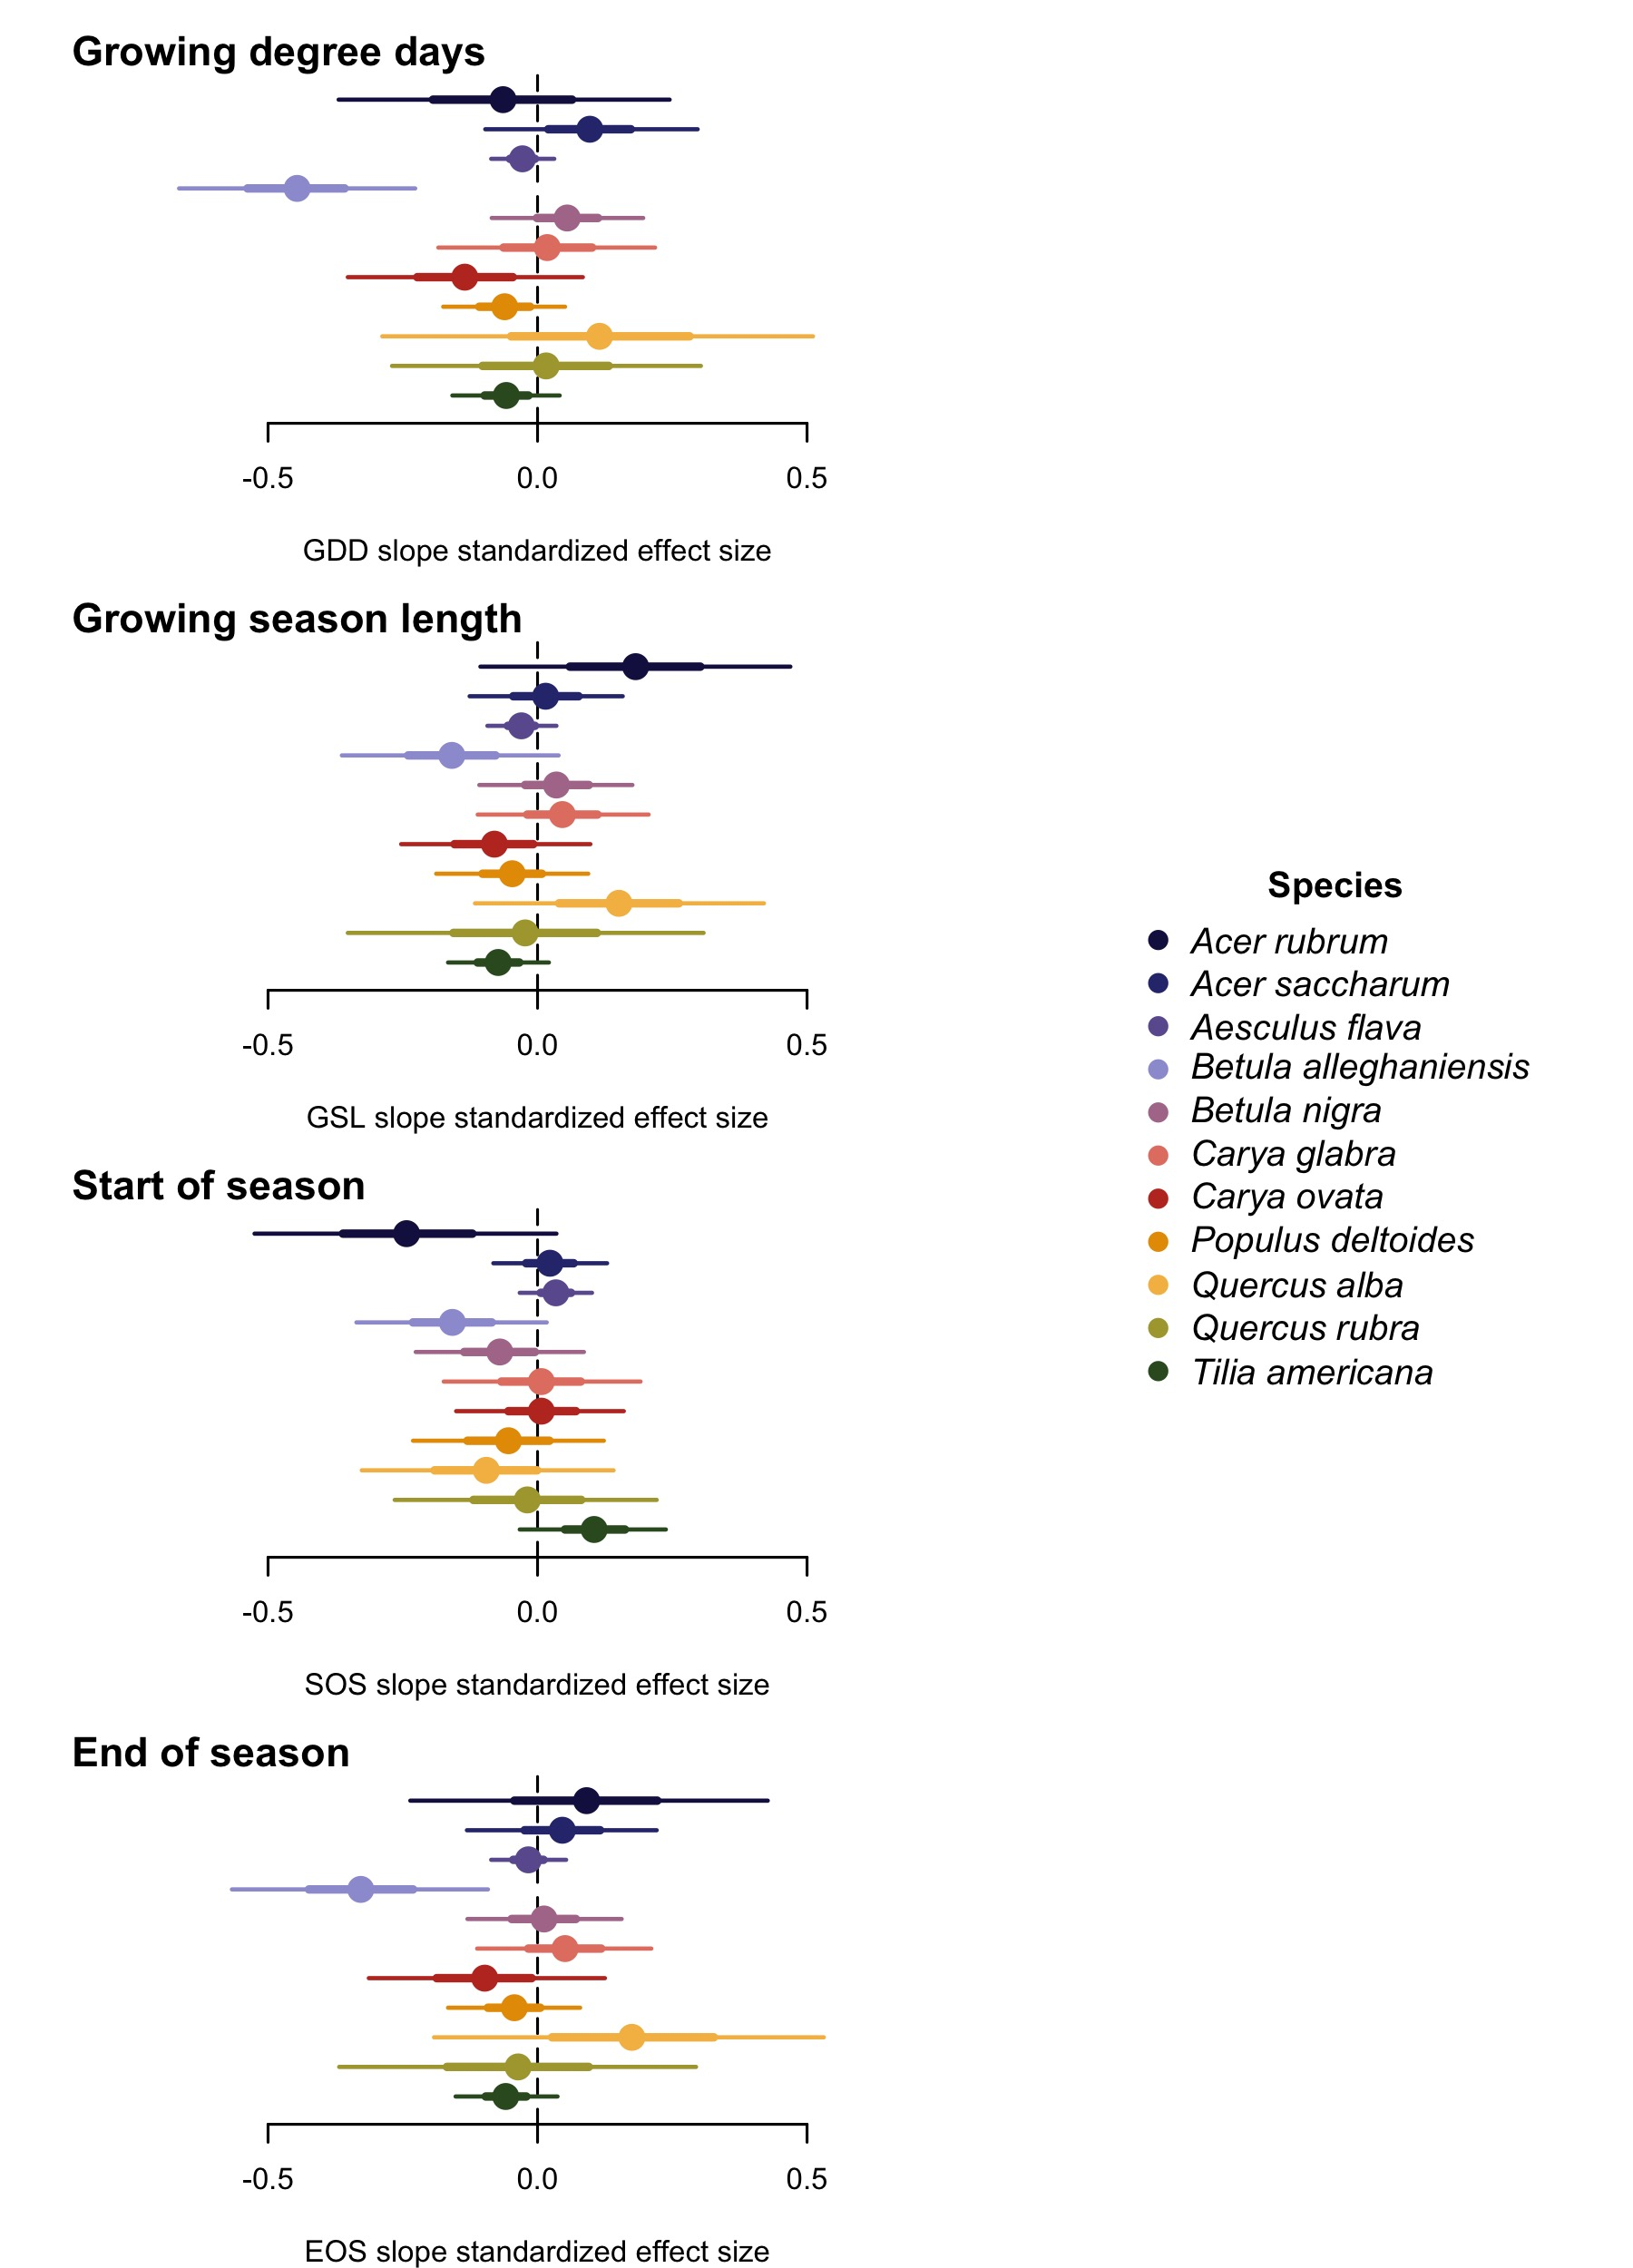
\includegraphics[width=0.8\textwidth]{../../analyses/figures/growthModelsMain/zscored/muALLbspp.pdf}
% \caption{Standardized (z-scored) slope estimates for Coringtreespotters. The dots represent the mean of the posterior distribution, the thick lines the 50\% uncertainty intervals (UI) and the thinner lines, the 90\% UI.}
% \label{fig:bsppZscored}
% \end{figure}

\end{document}
